\documentclass{exam}
\usepackage{preamble}
\pagestyle{headandfoot}
\firstpageheader{Physics}{Unit 2: Acceleration}{Test}

\CorrectChoiceEmphasis{\color{red}\bfseries}
\SolutionEmphasis{\color{red}}
\printanswers



\begin{document}
\begin{questions}

\question
What is average acceleration?

\begin{choices}
    \choice change in velocity divided by change in position
    \correctchoice change in velocity divided by change in time
    \choice rate of change of displacement
    \choice rate of change of position
\end{choices}

\question
Acceleration may be measured in units of \fillin\ .

\begin{choices}
    \choice meters per second (\SI{}{m/s})
    \correctchoice meters per second squared (\SI{}{m/s^2})
    \choice meters squared per second (\SI{}{m^2/s})
    \choice seconds (s)
\end{choices}

\question
If a falcon is flying at \SI{10}{m/s} and then, some short time later, flies at \SI{17}{m/s}, what is the falcon's change in velocity?

\begin{choices}
    \choice It's not possible to know without knowing the change in time.
    \choice \SI{10}{m/s}
    \choice \SI{17}{m/s}
    \correctchoice \SI{7.0}{m/s}
\end{choices}

\question
Amanda jogs with a constant velocity of \SI{6.2}{m/s} for 3.0 seconds. What is her average acceleration?

\begin{choices}
    \choice \SI{2.06}{m/s^2}
    \choice \SI{0.48}{m/s^2}
    \choice \SI{6.2}{m/s^2}
    \correctchoice \SI{0.0}{m/s^2}
\end{choices}

\question % Like Ch2 #18
The velocity of an airplane increases from 0 to \SI{36}{m/s} in \SI{12}{s}. What is the plane's average acceleration?

\begin{choices}
\choice \SI{0.333}{m/s^2}
\CorrectChoice \SI{3.0}{m/s^2}
\choice \SI{36}{m/s^2}
\choice \SI{432}{m/s^2}
\end{choices}

\question
An object moves in accordance with the graph below. What is the object's acceleration?
\vspace{1em}

\begin{minipage}{0.3\textwidth}
    \begin{choices}
    \choice \SI{1}{m/s^2}
    \choice \SI{6}{m/s^2}
    \choice \SI{125}{m/s^2}
    \CorrectChoice \SI{5}{m/s^2}
    \end{choices}
\end{minipage}%
\begin{minipage}{0.3\textwidth}
    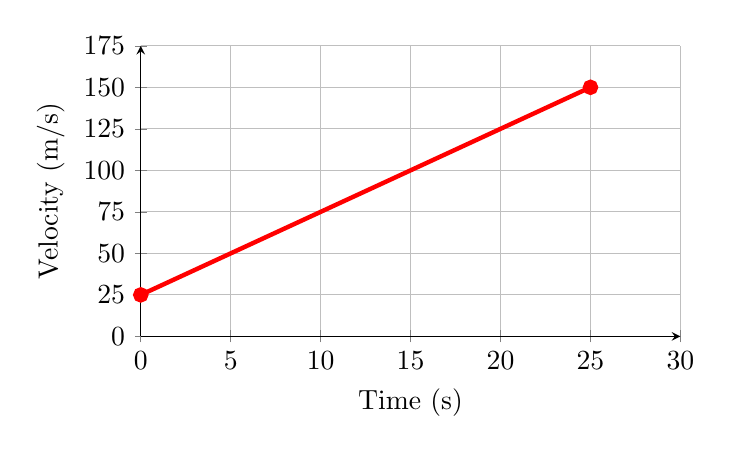
\begin{tikzpicture}
    \begin{axis}[width=240pt, height=150pt,
    axis y line=left, 
        axis x line=left,
        ymin=0, ymax=175,
        xmin=0, xmax=30,
        ylabel = Velocity (m/s),
        xlabel = Time (s),
        grid=both,
        ytick={0,25,...,175}
    ]
    \addplot[
        %color=green!67!black,
        color=red,
        mark options={color=red},mark=*,
        ultra thick,
        ]
        coordinates {
        (0,25)(25,150)
        };
    \end{axis}
    \end{tikzpicture}
\end{minipage}


\question
The velocity vs.~time graph represents the motion of a bicyclist. What is their acceleration?

\begin{minipage}{0.3\textwidth}
    \begin{choices}
        \choice \SI{25}{m/s^2}
        \correctchoice \SI{2}{m/s^2}
        \choice \SI{50}{m/s^2}
        \choice \SI{5}{m/s^2}
    \end{choices}
\end{minipage}%
\begin{minipage}{0.3\textwidth}
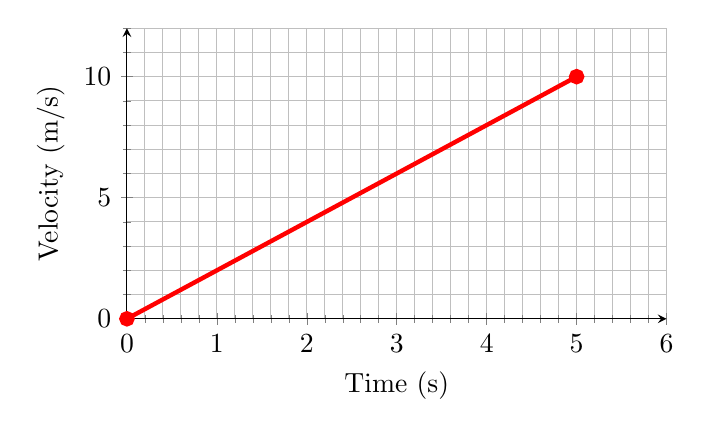
\begin{tikzpicture}
\begin{axis}[width=240pt, height=150pt,
        axis y line=left, 
        axis x line=left,
        ymin=0, ymax=12,
        xmin=0, xmax=6,
        ylabel = Velocity (m/s),
        xlabel = Time (s),
        grid=both,
        ytick={0,5,...,15},
        yminorgrids=true, minor y tick num=4,
        xminorgrids=true, minor x tick num=4,
    ]
    \addplot[
        color=red,
        mark options={color=red},mark=*,
        ultra thick,
        ]
        coordinates {
        (0,0)(5,10)
        };
\end{axis}
\end{tikzpicture}     
\end{minipage}

\question
What is the acceleration of an object whose motion is shown by the graph below?

\begin{minipage}{0.3\textwidth}
    \begin{choices}
        \choice \SI{-52.5}{m/s^2}
        \choice \SI{3}{m/s^2}
        \choice \SI{52.5}{m/s^2}
        \correctchoice \SI{-3}{m/s^2}
    \end{choices}
\end{minipage}%
\begin{minipage}{0.3\textwidth}
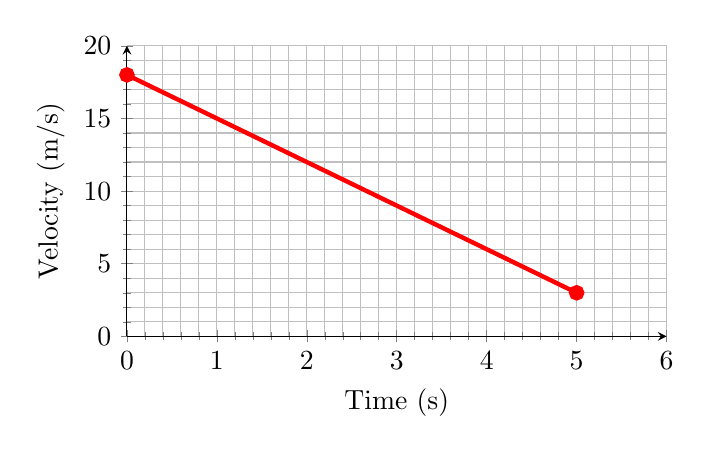
\begin{tikzpicture}
\begin{axis}[width=240pt, height=150pt,
        axis y line=left, 
        axis x line=left,
        ymin=0, ymax=20,
        xmin=0, xmax=6,
        ylabel = Velocity (m/s),
        xlabel = Time (s),
        grid=both,
        ytick={0,5,...,20},
        yminorgrids=true, minor y tick num=4,
        xminorgrids=true, minor x tick num=4,
    ]
    \addplot[
        color=red,
        mark options={color=red},mark=*,
        ultra thick,
        ]
        coordinates {
        (0,18)(5,3)
        };
\end{axis}
\end{tikzpicture} 
\end{minipage}

\question
Mario the soccer player jogs in one direction at a constant velocity in accordance with the graph below. What is his displacement?

\begin{minipage}{0.3\textwidth}
    \begin{choices}
        \choice \SI{0.0}{m}
        \correctchoice \SI{56}{m}
        \choice \SI{7}{m}
        \choice \SI{15}{m}
    \end{choices}
\end{minipage}%
\begin{minipage}{0.3\textwidth}
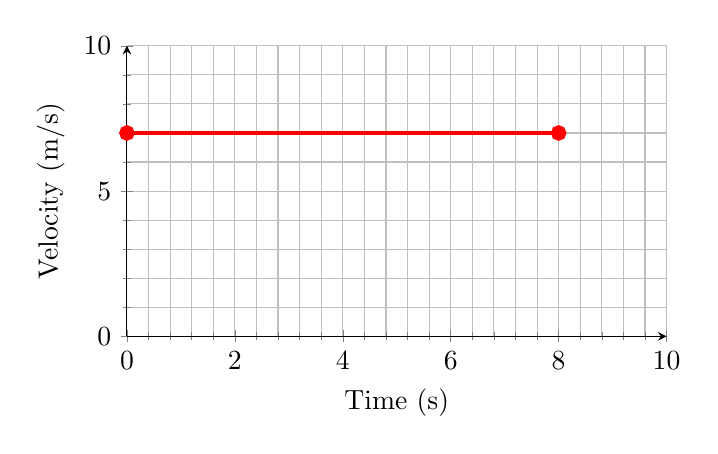
\begin{tikzpicture}
\begin{axis}[width=240pt, height=150pt,
        axis y line=left, 
        axis x line=left,
        ymin=0, ymax=10,
        xmin=0, xmax=10,
        ylabel = Velocity (m/s),
        xlabel = Time (s),
        grid=both,
        ytick={0,5,...,10},
        % ymajorgrids=true,
        % xmajorgrids=true,
        yminorgrids=true, minor y tick num=4,
        xminorgrids=true, minor x tick num=4,
    ]
    %\fill[black!20] (axis cs: 0,0) rectangle (axis cs: 6,15);
    \addplot[
        color=red,
        mark options={color=red},mark=*,
        ultra thick,
        ]
        coordinates {
        (0,7)(8,7)
        };
\end{axis}
\end{tikzpicture}
\end{minipage}

\question
An object's motion is represent by the graph below. What is the object's displacement?

\begin{minipage}{0.3\textwidth}
    \begin{choices}
        \correctchoice \SI{-15}{m}
        \choice \SI{15}{m}
        \choice \SI{-105}{m}
        \choice \SI{105}{m}
    \end{choices}
\end{minipage}%
\begin{minipage}{0.3\textwidth}
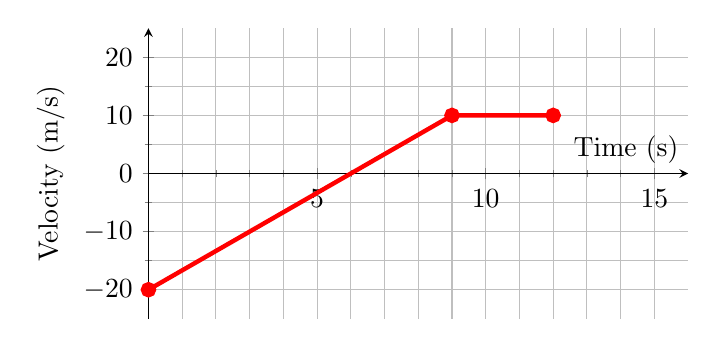
\begin{tikzpicture}
\begin{axis}[width=240pt,height=150pt,
    axis y line=left, 
    axis x line=center,
    xlabel = Time (s),
    ylabel = Velocity (m/s),
    ymin=-25, ymax=25,
    xmin=0, xmax=16,
    ytick={-20,-10,...,20},
    xtick={0,5,...,15},
    ymajorgrids=true,
    xmajorgrids=true,
    yminorgrids=true, minor y tick num=1,
    xminorgrids=true, minor x tick num=4,
    % x label style={anchor=west},
    clip=false,
]
    \addplot[
        %color=green!67!black,
        color=red,
        mark options={color=red},mark=*,
        ultra thick,
        ]
        coordinates {
        (0,-20)
        (9,10)
        (12,10)
        };
\end{axis}
\end{tikzpicture}
\end{minipage}

\end{questions}
\end{document}